%% Support sites:
%% http://www.michaelshell.org/tex/ieeetran/
%% http://www.ctan.org/tex-archive/macros/latex/contrib/IEEEtran/
%% http://www.ieee.org/

% The testflow support page is at:
% http://www.michaelshell.org/tex/testflow/

\documentclass[journal]{IEEEtran}

%\usepackage{blindtext}
\usepackage{graphicx}
\usepackage{cite}
\usepackage{float}
% correct bad hyphenation here
\hyphenation{op-tical net-works semi-conduc-tor}

%\renewenvironment{titlepage}
%{}

\title{Do No Harm: Are Rainbow Colormaps Dangerous? \\}
\author{Derek~Miller \\ Brigham Young University}% <-this % stops a space


\begin{document}

% make the title area
\begin{titlepage}
\maketitle
\thispagestyle{empty}
%\vspace*{\fill}

\begin{abstract}
This document addresses the controversies and contradictions
surrounding colormaps using a rainbow color scheme in data visualization.
Colormaps are used frequently in science and its applications
to display complex data sets by
representing data points as colors on a spectrum. The scientific
community is divided on whether the default 'jet' or rainbow colormap
is best for data visualization. Some point to evidence in medical imaging
that suggests the rainbow colormap distorts data, resulting in slower and 
less accurate data interpretation. Others have shown that the
scientific community is used to reading graphics with rainbow
color schemes and are no less accurate than others who use
a different color scheme. This document finds that rainbow colormaps
are generally inferior to perceptually uniform colormaps. However, it
seems that rainbow colormaps are not the main cause of diagnostic error,
though there is sufficient evidence showing that diagnostic errors do occur.
To avoid errors in data interpretation, some scientific software programs
have changed their default colormap away from the rainbow scheme.
Nevertheless, many find the rainbow colormap to be aesthetically pleasing
and continues to be used extensively in medical imaging.
\end{abstract}
\tableofcontents
\vspace*{\fill}
\end{titlepage}

\IEEEpeerreviewmaketitle

\section{Introduction}
Scientific progress depends on the proper evaluation
of evidence from data. The evaluation process usually
starts by visualizing data produced from an experiment
or procedure. For example, a radiologist determines the
type and severity of a bone fracture by looking at an
image representation of X-ray data.
Data sets with one or two variables are generally easy to visualize. 
When a data set has three or more variables, it is much harder to show all the variables
on one visualization. Color is commonly used to show three or more variables in one visualization.

A common way to represent data with color is by using a
colormap---a function that assigns data points to
an ordering of colors. Nathaniel Smith
calls colormaps ``an interface between the data and your
brain \cite{viridis}.'' A scientist interested in visualizing a
data set must choose a colormap that reflects the nature of the data. 
When judiciously chosen, colormaps reveal hidden structure that would go unnoticed
otherwise. A careless colormap selection, on the other hand, may distort the data and
lead viewers to misinterpret the data. This can have
serious consequences, especially in medicine and public health.
Doctors rely on visualization software to interpret medical
data correctly and properly diagnose and treat disease.
Public health policy is also decided based on data often presented 
in visual form. While scientists agree that data analysis
should be rigorous, consistent, and reproducible, many disagree over the proper
use of color in data visualization---especially rainbow colormaps.

Despite visually distorting the data, many scientists
prefer a rainbow color scheme for its aesthetic appeal
and historical use in scientific publications. This literature
review explores the advantages and disadvantages
of rainbow colormaps, why they are preferred by some
scientists and discouraged by others, and how spectral color schemes are used
in applied data analysis. First, this review gives a basic summary 
of the color theoretic properties of rainbow colormaps. Then, it will
address color perception issues of spectral color schemes, including
color vision impairment. Finally, rainbow colormap applications are discussed
in medical imaging and cartography.

\section{Colormap Fundamentals}

To represent data as color, the data must first be converted into RGB values by way of 
a colormap. The computer then turns the RGB values into light, projected from a screen.
When the light reaches our eyes, photorecpetors called cones detect certain wavelengths
of light and send that information to the brain. The brain then interprets the information
and generates the perception we call color \cite{viridis}.
To avoid ambiguity when talking about color, scientists use
color models---abstract mathematical representations that
describe a color as a collection of numbers.


\subsection{Color Models and Spaces}

When a color model is used to produce color on a specific medium, the resulting set
of colors is called a color space. For example, the RGB model
describes color as the combination of red, green, and
blue light. A computer screen renders color using the
RGB model, thus the color produced by digital screens
with the RGB model is a color space. Another example is the
CMYK model, which describes color as combinations of
cyan, magenta, yellow, and black. Printers produce colors using this model.
\cite{colormapping}. The combination of cyan, magenta, yellow, and black
ink on a specific printer constitutes a color space. The selection and modification of color
models and spaces happens before colormaps or data visualizations can be created. 

Most color spaces produce a similar set of colors. However, there are some colors
that do not translate well between color spaces. For example, consider the image
shown in Figure 1 and Figure 2. When this document is viewed digitally, the colors will look
different than the colors on a printed copy. This represents
a transformation from an RGB color space to a CMYK color space \cite{colorvblackwhite}.
Color changes when transformed. This is the motivation for developing perceptually
uniform color models, as in the CIECAM02-UCS color model. Good models of color
distance may not preserve absolute color, but perceived color difference tends
to remain the same across all media \cite{ciecam02}. Perceptually uniform colormaps
can be produced using these models \cite{viridis}. In general, rainbow colormaps
are not perceptually uniform because the lightness is not consistent.

This has not stopped some from attempting to modify---and therefore preserve---the
rainbow colormap. The adjustments refer to the Munsell color specification system,
which describes color with hue, saturation, and lightness. ``This system
divides up the colors humans are capable of perceiving
into equal perceptual divisions of color lightness and
color saturation for each color hue. \cite{colormapping}''
Hue refers to the attribute generally associated with the color name (i.e. red,
orange, yellow, green, blue). On a color wheel, hue is the position of the color
on the color wheel. Saturation is the intensity of the hue. In
physical terms, it is the purity of the light wave frequency. Lightness is the
amount of light emitted by a color. Low lightness results in a darker color;
high lightness results in a lighter color. \cite{colorguidelines}.
Sisneros et al created a colormap modification framework that smooths the variation
in luminance (or lightness) and chromaticity, which is a combination of saturation
and hue. Their method can be applied to any perceptually non-uniform colormap.
However, they focused their efforts on improving the rainbow colormap, since it is still widely
used in science. Their improved rainbow colormap contains subdued colors that better
represent image data \cite{chasingrainbows}. 

\subsection{Color Schemes}

There are three main types of color schemes that define a colormap.
Sequential color schemes vary in lightness but do not
vary in hue. If two sequential color schemes have different hues and are
connected at their lightest ends, it is called a diverging color scheme. Qualitative color
schemes vary in hues with little variation in lightness
and saturation \cite{colormapping}. The rainbow colormap uses a continuous,
qualitative color scheme. The images in Fig. 2
are examples of image data plotted with 
sequential, diverging, and rainbow colormaps.

\begin{figure}[H]
\centering
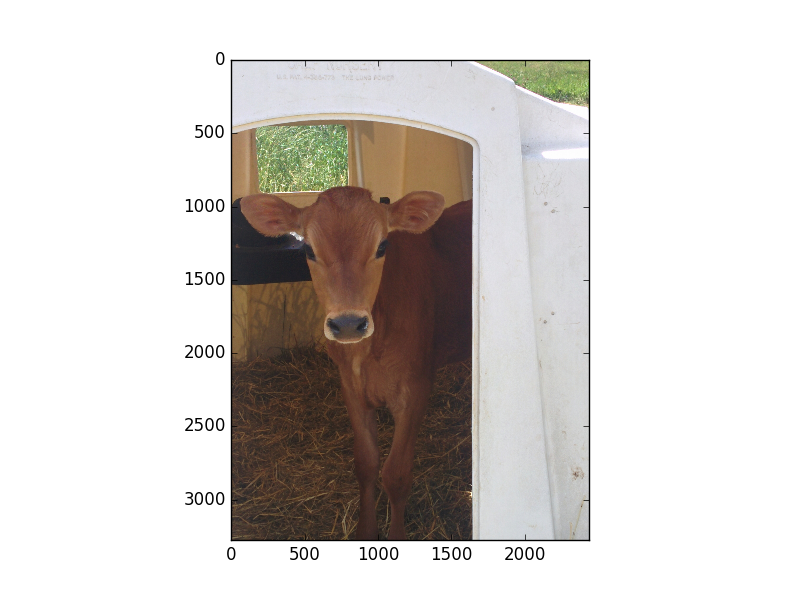
\includegraphics[width=1.1in]{calf_original}%
\caption{An image of a calf. This and corresponding images were created by the author.}
\end{figure}

\begin{figure}[H]
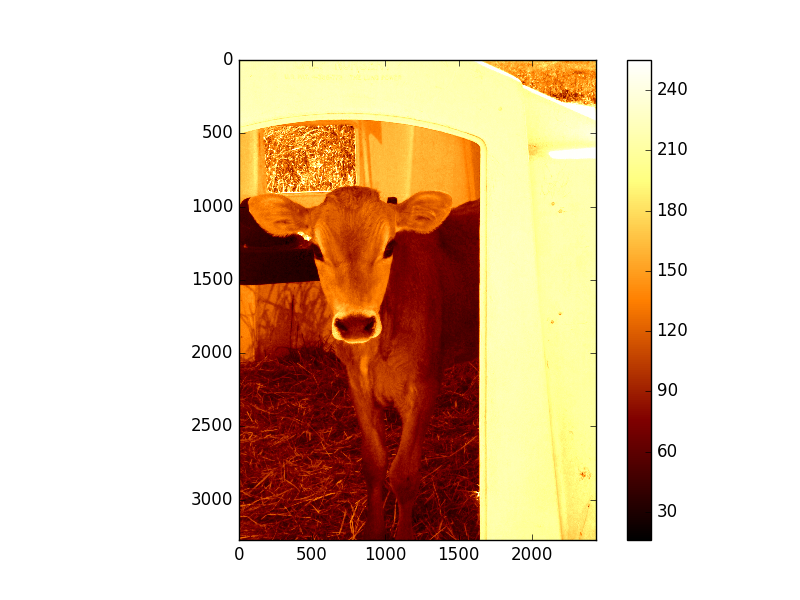
\includegraphics[width=1.1in]{calf_sequential}%
\hfil
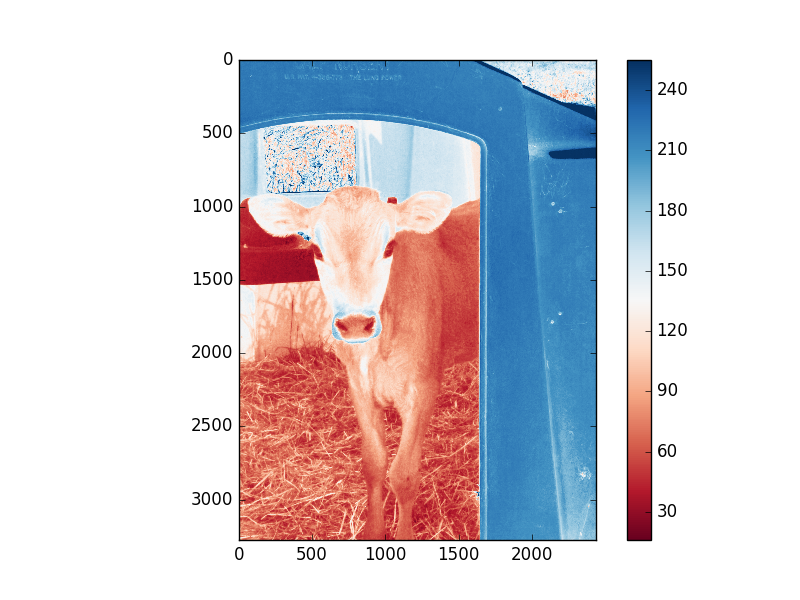
\includegraphics[width=1.1in]{calf_diverging}%
\hfil
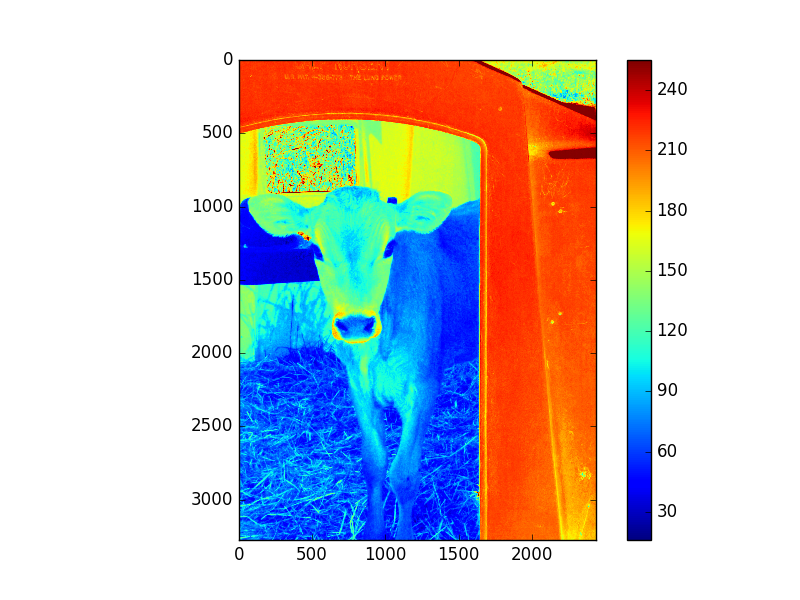
\includegraphics[width=1.1in]{calf_rainbow}%
\caption{The calf image plotted with a
sequential, diverging, and rainbow colormap.}
\end{figure}

\subsection{Colormaps}

The main problem when designing a colormap is that there is no natural ordering of the colors
from least to greatest. Some might argue that there is a natural
ordering---the brain's interpretation of the electromagnetic spectrum.
Based on light wave frequency, this color ordering is rainbow-like with respect
to the color hues \cite{colormapping}. It starts with red and on to orange,
yellow, green, blue, and so forth. This is the foundation for the rainbow colormap.
It was especially popular among physicists and soon grew to become the default
in many scientific software applications \cite{rainbowstill,matlab}. However,
this colormap was not created for data representation. It was designed based
on accurately representing light waves, not data.

What are the criteria for evaluating a colormap? Several authors have created
methods to evaluate color
choice. In one paper, color schemes are evaluated by
three variables of the CIELUV color model. The first
is color distance. The CIELUV model is designed to
measure distance between colors. If the distances are
equally spaced, that’s a good thing. Linear separation
is the second variable. It refers to “the ability to separate targets
from non-targets in the colour model being
used.” For example, suppose a doctor wants to identify
a tumor and uses a colormap to display the data. If the
colors are not linearly sepparable in the color model, it
will be more difficult to identify the tumor even if the
colors are mathematically different. The third variable
is color category. This refers to color regions in which
there are both target and non-target elements \cite{colorchoice}.
 These characteristics do not account for multidimensional data projected into two-dimensional
space. CheckViz attempts to account for this problem
by using a perceptually uniform color coding so that
distortions such as those described above are accounted for when 
scientists want to visualize multidimensional data \cite{checkviz}.
The specific criteria of the color
model and color space must reflect the attributes of the colormap.
\par
Sometimes, when color encodings are converted to
grayscale, it can alter the perception of the data. There
are many algorithms to cast a color encoding to grayscale.


Colormaps have a variety of properties that make them unique and potentially
useful. However, there is controversy among scientists and visualization
experts over certain properties of the rainbow colormap. First, the rainbow
gradient is not a perceptually consistent ordering of colors. Similarly, it
is not perceptually uniform as the variation in lightness is inconsistent.
Finally, the rainbow colormap traverses through many
highly saturated colors in color space.


There are multiple advantages to using rainbow colormaps. For one,
it is clear that users tend to prefer it
over other colormaps for its aesthetic appeal
\cite{spectralschemes, choropleth, endofrainbow}. 
The variety in hue also can accentuate relationships in the data than
a sequential, single-hue colormap. History is an advantage.
\par
However, the advantages can also be disadvantages.
When accentuating relationships, a human interpreter
might see signal where there is none. This seems to be
what happens when the data lie in certain regions (as in
between blue green and yellow) \cite{colorchoice}.
\par
Readers of scientific literature will recognize the rainbow colormap. 
It appears often in scientific publications and has 
broad appeal in the scientific community
\cite{endofrainbow, rainbowstill, spectralschemes,choropleth}.
 Historically, rainbow colormaps like
MATLAB’s ‘jet’ have been the default colormaps used
in data-handling software \cite{matlab}. Despite its prevalence, 
many scientists oppose rainbow-gradient representations of data
\cite{rainbowstill, endofrainbow, viridis,arteryvis}.
 In one study, medical students were
asked to identify risk factors for heart disease in visualizations
of artery data. On average, the participants
using rainbow-colored visualizations took more time
and made more errors than participants using divergence-colored visualizations. 
Furthermore, the participants “thought they did well using the rainbow color
map even when in reality they did not perform as well
as the participants who used the diverging color map
\cite{arteryvis}.” This compelling evidence suggests
that the rainbow colormap is clearly inferior to other
colormaps.
\par
Others disagree. They claim that users have learned to
read data with the rainbow colormap and prefer its
aesthetic appeal \cite{spectralschemes, choropleth}. One
experiment tested data interpretation accuracy under
diverging, sequential, and spectral (rainbow) color
schemes. “Of 63 subjects who evaluated spectral and
sequential schemes, 56 percent selected spectral as the
best...We had expected the spectral scheme to interfere
with map-reading accuracy and with understanding
map patterns, but this did not occur,” Brewer writes.
“Our subjects preferred the spectral scheme
and performed well with it \cite{spectralschemes}.”
 While the rainbow colormap did not outperform other colormaps, it
appears to do no harm. Users can accurately interpret
rainbow-colored data visualizations.

\section{Color Perception}

One of the advantages of using perceptually uniform colormaps is
that they show the data accurately even if the colors do not appear
the same. Color perception can change for a number of reasons. When 
colors are placed near each other, it changes the way our eyes see that color.
The brain adjusts the amount of light that enters the eyes based
on external conditions. For example, colors appear more bright under diffused
light. Competing bright colors also diminishes the overall perception
of their brightness.

\subsection{Choosing Colors}

Mark Rothko and Josef Albers are notable artists who explored the human relationship
with color perception. Some colors blend together while others almost appear to be in
conflict with each other, causing a perceived vibration in the colors.

Another example of color perception under different conditions is the 
color-of-the-dress meme that became popular in 2015. The picture was
sent on social media sites asking whether the dress was black and blue
or white and gold. This effect happens because our eyes perform a kind 
of normalization under different light conditions. This adjustment alters
the perception of what the colors look like \cite{viridis}. Other examples from psychology 
place the same color in two images with different colors surrounding the
color being studied. Even though the colors are the same, they appear to be 
different because of the context that they are in. This means that sometimes
we see color differences even when there are none.

\subsection{Perceptual Uniformity}

Other times, color differences can't be detected easily or at all. This is 
especially common among people who have some form of color vision impairment,
as in colorblindness. The estimated colorblind population is somewhere around 5-8\%
and affects mostly males of European descent \cite{colormapping}.

Colorblindness results in colors falling on confusion lines---lines in which it
is difficult or impossible to distinguish between two colors \cite{colormapping}. People with full
color vision also have confusion lines and so in some sense are colorblind because 
we can't see the entire spectrum of light as colors. However, color deficient viewers
are special in that they do not see the normal range of colors as their peers.
There are multiple kinds of colorblindness.
Full color deficiency results in black and white vision and is very rare.
The most common form of color deficiency results in confusing shades of red and green \cite{colorchoice}.
%An example of a map colored with bright orange and green and what a deutoronome
%would see is given in Figure 3.

\subsection{Colorblindness}

For these genetic color deficiencies, it seems reasonable to design data
visualizations with colorblindness in mind. Unfortunately for the rainbow colormap,
the colors that a colorblind user sees are not the same as those seen by a person
with full color vision. Especially for high values, which are displayed in reds,
the variation in green is not easy to interpret for colorblind viewers \cite{cvimap}. In fact,
though they are aesthetically pleasing, people are slower at interpreting data with
large variations in color and make more errors \cite{arteryvis}. Yet, colorblind people still seem
to get by fine.

Color deficient viewers use clues to distinguish between colors that easily confuse them.
Brewer has conducted extensive research into how color deficient
viewers interpret color-encoded information. She has suggested several ways in which 
maps and information visualizations can be designed to help color deficient viewers.
A common theme in her research, as well as others, is that colormaps are greatly
improved when the dark-to-light variation is controlled and used to show progression \cite{cvimap}.
This is the idea behind perceptually uniform colormaps. Even when converted to black
and white, the visuals still preserve the nature of the data and are easy to interpret.



%
%[mapcvi]
%[simultaneouscontrast]
%[ciecam02]
%[mapguidelines]
%[colorvblackwhite]
%[colormapping]

\section{Applications}

The controversy surrounding the rainbow colormap does not appear to be random.
Certain industries disagree on how much the rainbow colormap should be 
discouraged. There is general agreement that rainbow colormaps are not as 
precise as perceptually uniform colormaps in representing data 
\cite{blackvwhite}. However, this 
does not mean that rainbow colormaps are discouraged in all cases
 \cite{spectralschemes}. 
Among the many uses of the rainbow colormap in the
literature, the two most cited are
medical imaging and cartography. Both care deeply about the use of color in 
their respective fields \cite{colorguidelines, standardmedimg}. Even within
 these applications, the recommended use of the rainbow colormap differs
 depending on the context.
 
\subsubsection{Cartography}

Maps are used to show public health information, the spread of disease, weather
forecasts, and other demographic data. This information is important to
 public policy and public awareness. This information is almost always shown
 using color. Choosing an appropriate color scheme is not a trivial task. In her
article \textit{Mapping Mortality: Evaluating Color Schemes for Choropleth
Maps}, Cynthia Brewer shows that a judicious choice of color is ``worth 
the extra effort and expense'' because ``it permits greater accuracy in map
reading \cite{choropleth}.'' For public understanding of data, the rainbow colormap
seems to do no harm and users tend to prefer it.

Rainbows are not always good for maps, however. An assortment of colormaps were
developed and shown to be superior to rainbow schemes when used for oceaonography.
Sea level is an important metric in these contexts and a rainbow colormap poorly 
represents the coastline where land and sea meet. In this context, customized colormaps
outperform most other colormaps \cite{oceanography}. In contexts where the data are in a particular form
that the scientist knows, it is best to create a customized colormap that gives 
more accurate results.

\subsubsection{Medical Imaging}

The consequences for color misuse in medical imaging are more severe. Research
already shows that the potential for diagnostic errors increases when 
rainbow color schemes are used \cite{arteryvis}. In this research, color may not
be necessary and only used for convenience. However, some procedures require 
medical images that must be interpreted using color. In this case, it
is especially important that hardware components be standardized so that color
can be interpreted effectively. Since there are many manufacturers that produce
image processing software and display hardware, there is no consensus which 
color models or color mappings should be used by the medical community.
The Summit on Color in Medical Imaging
met to reach a consensus on how to standardize color use 
\cite{standardmedimg}. Images that are important to medicine but not exclusively
part of the community would not be held to these standards.

Bioinformatics and genetics are two fields related to medicine that 
could be exempt from the standards set in medical imaging. In fact, many tools
are being created now to analyze the vast amount of data that can be collected
in genetics. One such tool uses clustering techniques to find biomarkers in 
gene data. This software is written in Matlab and designed to run on Microsoft
Windows and Linux x86 \cite{marvis}. This specific choice of software uses an
older version of Matlab and uses the \textit{jet} default colormap. 
Software updates and hardware limitations make it difficult to change 
the visualization system. This may be another reason why doctors prefer
the rainbow visualization---it is just too difficult to change.

Many recognize that change is not easy. Some recommend changing 
colormap defaults instead of setting standards \cite{viridis}. That way, some 
consistency can be maintained while still allowing a little variation in the
implementation. This is the goal of visualization studies like the one 
carried out in the development of the HemoVis medical imaging program 
\cite{arteryvis}. This is especially important because it is not feasible for
every software to be written independently without dependencies on other
software.

\section{Conclusion}

Color is still an essential attribute of data visualizations. Representing data
with color is best done through a colormap designed specifically for the data in
mind.
Colormaps require a vast amount of knowledge to be thoroughly constructed. It 
involves disciplines as different as engineering, computer science, graphic design,
and psychology. The recent development in color rendering technology has made it 
possible to develop and test many different colormaps. In particular, it seems clear
the rainbow colormap has many undesirable properties when trying to represent data.
It takes more time for viewers to interpret data with this colormap and they tend to
make mistakes when the data fall in areas where the color changes do not match 
equivalent changes in the data. There does not seem to be a problem in cartography
and people tend to prefer the rainbow colormap because it is familiar and aesthetically pleasing.
Despite these preferences, there is an increasing movement to replace the rainbow
colormap as the default colormap in scientific software \cite{matlab}. Recommended
alternatives are colormaps that are more perceptually uniform than the rainbow 
colormap. The variety of colors is diminished and the darkness-to-lightness progression
is more consistent with human perception of color change.

When data must be represented using color, most recommend using a perceptually
uniform colormap because it more accurately represents the data and is more 
friendly to colorblind or color impaired individuals. When colors cannot be changed
to accomodate for color impairment, redundancy can be added to the visualization
so as to encode the same information the color represents as a small icon or by using
a different visual variable such as position or size. In contexts where data
interpretation is to be precise and time-efficient, scientists are discouraged from
using the rainbow colormap. In applications where user preferences are valued over representational accuracy, the rainbow colormap is acceptable. However, scientists
are encouraged to use perceptually uniform colormaps to phase out the rainbow colormap
as a default and replace it with a colormap that more accurately represents a larger
variety of data.


\ifCLASSOPTIONcaptionsoff
  \newpage
\fi

\section{Appendix}

The following is useful for understanding the development of 
colormaps and how the rainbow colormap came to be outdated.

\subsection{Trichromatic Theory}

This theory was developed by Thomas Young in 1802 and extended quantitatively by 
Hermann von Helmholtz in 1894. This was the first time that the photoreceptors
in the retina of the eye responded to three different wavelengths of light---long,
medium, and short \cite{colorimetry}. They were thought to respond to red, green, and blue light.

\subsection{Munsell Color Specification System and HSV/HSL}

This was developed by Albert Munsell in the early 20th century using paint chips.
This was one of the first systems to develop the concept that color is
made up of three independent variables---hue, chroma, and value or lightness.
Later developments added to this model and made the perception of color via
these attributes more concrete \cite{colormapping}. The model relies on cylindrical coordinates
of colors arranged by these variables. This development led to the more
widely known HSL/HSV model \cite{colorimetry}. These models draw inspiration from the Munsell system
and describe the perceptual attributes of color as combinations of hue,
saturation, and value or lightness.

\subsection{Commision Internationale de l'Eclairage (CIE)}

While the Munsell color system was a good way to describe the appearance of color,
there was no rigorous way to define a consistent way to create color. The Commision
Internationale de l'Eclairage (CIE) developed the RBG color specification system
and continued to develop reliable color models \cite{colorimetry}.

\subsubsection{CIEXYZ}

After the RGB color specification system, CIE developed the CIEXYZ model in 1931
which became widely accepted. It is still used today \cite{viridis}. It's development was 
focused on converting measurable, physical properties of light into a model
that represented human color perception by way of color matching experiments 
\cite{colorimetry}.
Since humans do not see all light 
as color, the model collapsed a large variety of light waves into a smaller 
spectrum that humans could see as color. This is the model typically used in 
generating a rainbow colormap.

\subsubsection{CIELUV and CIELAB}

The CIEXYZ color model is not a model of color distance. Thus, CIE set out to
define color distance and create a uniform color model based on that notion.
In 1976, CIE produced two uniform color models, CIELUV and CIELAB \cite{colorimetry}. Some colormaps,
like Matlab's \textit{perula} colormap, are designed to be perceptually
uniform in the CIELAB color space \cite{viridis}. While not 
completely uniform, they provided the best notion of perceptual uniformity until
the CIECAM-02 models were developed in 2002.

\subsubsection{CIECAM02}

In 2002, CIE released new develpments in perceptually uniform color models with
the CIECAM02 model family. CIE now recommends using the CIECAM02-UCS model 
\cite{ciecam02}.
One of the primary differences between CIELAB and CIECAM02-UCS is that the latter
is more perceptually uniform between similar colors than distant colors. CIELAB
is a good model of perceptual color distance for very different colors, but 
is not as good a model of the distance between similar colors.
CIECAM02-UCS The open source colormap \textit{viridis} created by Smith and van der Walt, uses
the CIECAM02-UCS color space to provide a perceptually uniform color space more
consistent with small differences in data values \cite{viridis}. There has been
little to no research on the effects of using this most recent model on colormap
development.


% trigger a \newpage just before the given reference
% number - used to balance the columns on the last page
% adjust value as needed - may need to be readjusted if
% the document is modified later
%\IEEEtriggeratref{8}
% The "triggered" command can be changed if desired:
%\IEEEtriggercmd{\enlargethispage{-5in}}

% references section
%\bibliography{IEEEabrv,../bib/paper}
\bibliographystyle{ieeetr}
\bibliography{litreview}

% that's all folks
\end{document}



